% Created by tikzDevice version 0.10.1 on 2017-10-30 17:28:48
% !TEX encoding = UTF-8 Unicode
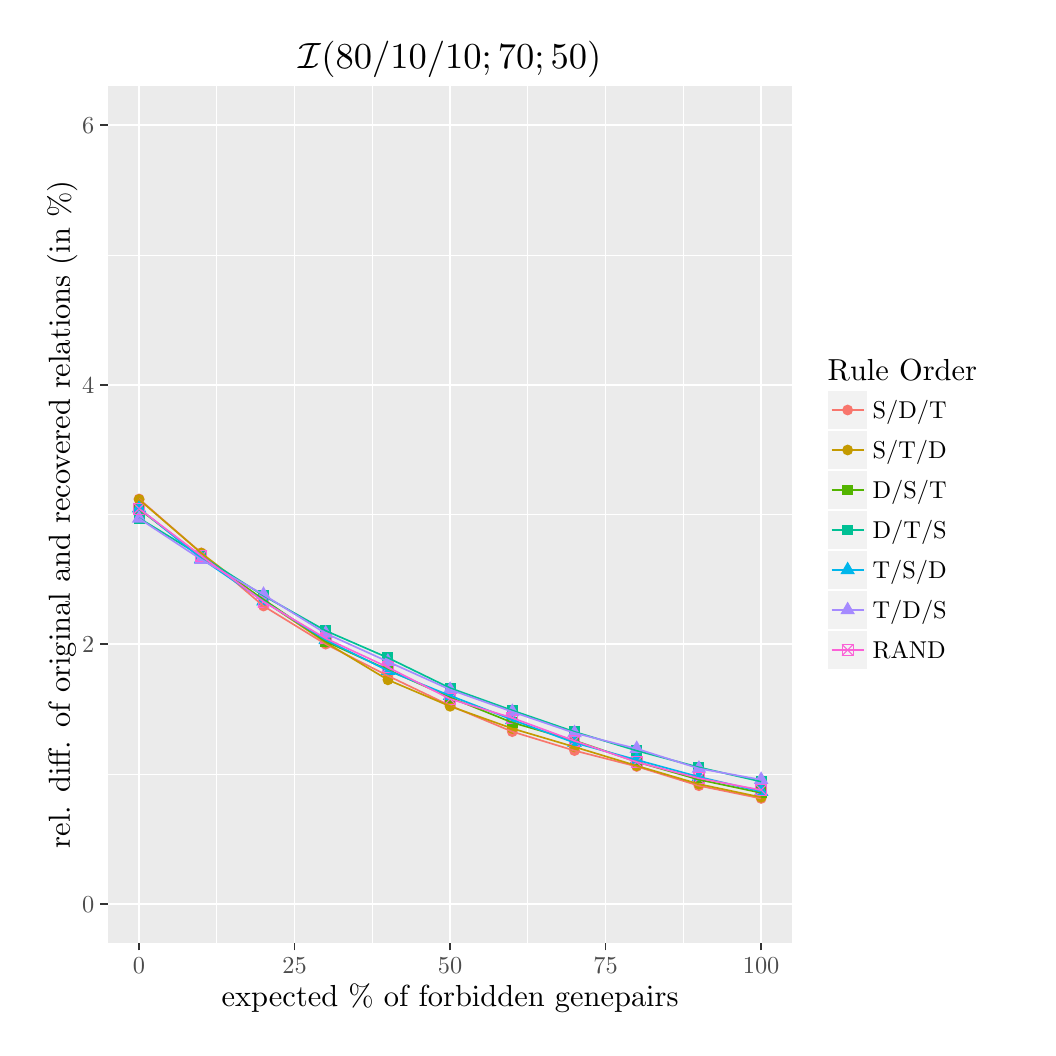
\begin{tikzpicture}[x=1pt,y=1pt]
\definecolor{fillColor}{RGB}{255,255,255}
\path[use as bounding box,fill=fillColor,fill opacity=0.00] (0,0) rectangle (361.35,361.35);
\begin{scope}
\path[clip] (  0.00,  0.00) rectangle (361.35,361.35);
\definecolor{drawColor}{RGB}{255,255,255}
\definecolor{fillColor}{RGB}{255,255,255}

\path[draw=drawColor,line width= 0.6pt,line join=round,line cap=round,fill=fillColor] (  0.00,  0.00) rectangle (361.35,361.35);
\end{scope}
\begin{scope}
\path[clip] ( 29.02, 30.69) rectangle (276.26,340.16);
\definecolor{fillColor}{gray}{0.92}

\path[fill=fillColor] ( 29.02, 30.69) rectangle (276.26,340.16);
\definecolor{drawColor}{RGB}{255,255,255}

\path[draw=drawColor,line width= 0.3pt,line join=round] ( 29.02, 91.64) --
	(276.26, 91.64);

\path[draw=drawColor,line width= 0.3pt,line join=round] ( 29.02,185.42) --
	(276.26,185.42);

\path[draw=drawColor,line width= 0.3pt,line join=round] ( 29.02,279.20) --
	(276.26,279.20);

\path[draw=drawColor,line width= 0.3pt,line join=round] ( 68.36, 30.69) --
	( 68.36,340.16);

\path[draw=drawColor,line width= 0.3pt,line join=round] (124.55, 30.69) --
	(124.55,340.16);

\path[draw=drawColor,line width= 0.3pt,line join=round] (180.74, 30.69) --
	(180.74,340.16);

\path[draw=drawColor,line width= 0.3pt,line join=round] (236.93, 30.69) --
	(236.93,340.16);

\path[draw=drawColor,line width= 0.6pt,line join=round] ( 29.02, 44.75) --
	(276.26, 44.75);

\path[draw=drawColor,line width= 0.6pt,line join=round] ( 29.02,138.53) --
	(276.26,138.53);

\path[draw=drawColor,line width= 0.6pt,line join=round] ( 29.02,232.31) --
	(276.26,232.31);

\path[draw=drawColor,line width= 0.6pt,line join=round] ( 29.02,326.09) --
	(276.26,326.09);

\path[draw=drawColor,line width= 0.6pt,line join=round] ( 40.26, 30.69) --
	( 40.26,340.16);

\path[draw=drawColor,line width= 0.6pt,line join=round] ( 96.45, 30.69) --
	( 96.45,340.16);

\path[draw=drawColor,line width= 0.6pt,line join=round] (152.64, 30.69) --
	(152.64,340.16);

\path[draw=drawColor,line width= 0.6pt,line join=round] (208.83, 30.69) --
	(208.83,340.16);

\path[draw=drawColor,line width= 0.6pt,line join=round] (265.03, 30.69) --
	(265.03,340.16);
\definecolor{fillColor}{RGB}{248,118,109}

\path[fill=fillColor] ( 40.26,191.06) circle (  1.96);

\path[fill=fillColor] ( 62.74,171.56) circle (  1.96);

\path[fill=fillColor] ( 85.22,152.35) circle (  1.96);

\path[fill=fillColor] (107.69,138.58) circle (  1.96);

\path[fill=fillColor] (130.17,127.15) circle (  1.96);

\path[fill=fillColor] (152.64,116.36) circle (  1.96);

\path[fill=fillColor] (175.12,106.96) circle (  1.96);

\path[fill=fillColor] (197.60,100.11) circle (  1.96);

\path[fill=fillColor] (220.07, 94.38) circle (  1.96);

\path[fill=fillColor] (242.55, 87.42) circle (  1.96);

\path[fill=fillColor] (265.03, 82.82) circle (  1.96);
\definecolor{fillColor}{RGB}{196,154,0}

\path[fill=fillColor] ( 40.26,190.85) circle (  1.96);

\path[fill=fillColor] ( 62.74,171.48) circle (  1.96);

\path[fill=fillColor] ( 85.22,154.29) circle (  1.96);

\path[fill=fillColor] (107.69,139.21) circle (  1.96);

\path[fill=fillColor] (130.17,125.68) circle (  1.96);

\path[fill=fillColor] (152.64,116.13) circle (  1.96);

\path[fill=fillColor] (175.12,108.10) circle (  1.96);

\path[fill=fillColor] (197.60,101.45) circle (  1.96);

\path[fill=fillColor] (220.07, 94.64) circle (  1.96);

\path[fill=fillColor] (242.55, 88.01) circle (  1.96);

\path[fill=fillColor] (265.03, 83.26) circle (  1.96);
\definecolor{fillColor}{RGB}{83,180,0}

\path[fill=fillColor] ( 38.30,185.41) --
	( 42.23,185.41) --
	( 42.23,189.33) --
	( 38.30,189.33) --
	cycle;

\path[fill=fillColor] ( 60.78,168.25) --
	( 64.70,168.25) --
	( 64.70,172.18) --
	( 60.78,172.18) --
	cycle;

\path[fill=fillColor] ( 83.25,152.77) --
	( 87.18,152.77) --
	( 87.18,156.69) --
	( 83.25,156.69) --
	cycle;

\path[fill=fillColor] (105.73,137.60) --
	(109.65,137.60) --
	(109.65,141.52) --
	(105.73,141.52) --
	cycle;

\path[fill=fillColor] (128.21,127.37) --
	(132.13,127.37) --
	(132.13,131.29) --
	(128.21,131.29) --
	cycle;

\path[fill=fillColor] (150.68,117.36) --
	(154.61,117.36) --
	(154.61,121.28) --
	(150.68,121.28) --
	cycle;

\path[fill=fillColor] (173.16,108.28) --
	(177.08,108.28) --
	(177.08,112.21) --
	(173.16,112.21) --
	cycle;

\path[fill=fillColor] (195.63,101.79) --
	(199.56,101.79) --
	(199.56,105.71) --
	(195.63,105.71) --
	cycle;

\path[fill=fillColor] (218.11, 94.09) --
	(222.04, 94.09) --
	(222.04, 98.02) --
	(218.11, 98.02) --
	cycle;

\path[fill=fillColor] (240.59, 87.66) --
	(244.51, 87.66) --
	(244.51, 91.58) --
	(240.59, 91.58) --
	cycle;

\path[fill=fillColor] (263.06, 82.90) --
	(266.99, 82.90) --
	(266.99, 86.83) --
	(263.06, 86.83) --
	cycle;
\definecolor{fillColor}{RGB}{0,192,148}

\path[fill=fillColor] ( 38.30,182.17) --
	( 42.23,182.17) --
	( 42.23,186.09) --
	( 38.30,186.09) --
	cycle;

\path[fill=fillColor] ( 60.78,168.43) --
	( 64.70,168.43) --
	( 64.70,172.36) --
	( 60.78,172.36) --
	cycle;

\path[fill=fillColor] ( 83.25,154.14) --
	( 87.18,154.14) --
	( 87.18,158.06) --
	( 83.25,158.06) --
	cycle;

\path[fill=fillColor] (105.73,141.46) --
	(109.65,141.46) --
	(109.65,145.39) --
	(105.73,145.39) --
	cycle;

\path[fill=fillColor] (128.21,131.70) --
	(132.13,131.70) --
	(132.13,135.63) --
	(128.21,135.63) --
	cycle;

\path[fill=fillColor] (150.68,120.76) --
	(154.61,120.76) --
	(154.61,124.69) --
	(150.68,124.69) --
	cycle;

\path[fill=fillColor] (173.16,112.67) --
	(177.08,112.67) --
	(177.08,116.60) --
	(173.16,116.60) --
	cycle;

\path[fill=fillColor] (195.63,104.95) --
	(199.56,104.95) --
	(199.56,108.87) --
	(195.63,108.87) --
	cycle;

\path[fill=fillColor] (218.11, 98.14) --
	(222.04, 98.14) --
	(222.04,102.06) --
	(218.11,102.06) --
	cycle;

\path[fill=fillColor] (240.59, 92.12) --
	(244.51, 92.12) --
	(244.51, 96.04) --
	(240.59, 96.04) --
	cycle;

\path[fill=fillColor] (263.06, 86.95) --
	(266.99, 86.95) --
	(266.99, 90.87) --
	(263.06, 90.87) --
	cycle;
\definecolor{fillColor}{RGB}{0,182,235}

\path[fill=fillColor] ( 40.26,190.74) --
	( 42.91,186.17) --
	( 37.62,186.17) --
	cycle;

\path[fill=fillColor] ( 62.74,172.56) --
	( 65.38,167.98) --
	( 60.10,167.98) --
	cycle;

\path[fill=fillColor] ( 85.22,157.20) --
	( 87.86,152.62) --
	( 82.57,152.62) --
	cycle;

\path[fill=fillColor] (107.69,143.17) --
	(110.33,138.60) --
	(105.05,138.60) --
	cycle;

\path[fill=fillColor] (130.17,132.06) --
	(132.81,127.49) --
	(127.53,127.49) --
	cycle;

\path[fill=fillColor] (152.64,123.04) --
	(155.29,118.47) --
	(150.00,118.47) --
	cycle;

\path[fill=fillColor] (175.12,114.30) --
	(177.76,109.72) --
	(172.48,109.72) --
	cycle;

\path[fill=fillColor] (197.60,106.01) --
	(200.24,101.44) --
	(194.95,101.44) --
	cycle;

\path[fill=fillColor] (220.07, 99.82) --
	(222.72, 95.25) --
	(217.43, 95.25) --
	cycle;

\path[fill=fillColor] (242.55, 93.68) --
	(245.19, 89.11) --
	(239.91, 89.11) --
	cycle;

\path[fill=fillColor] (265.03, 88.36) --
	(267.67, 83.78) --
	(262.38, 83.78) --
	cycle;
\definecolor{fillColor}{RGB}{165,138,255}

\path[fill=fillColor] ( 40.26,187.04) --
	( 42.91,182.46) --
	( 37.62,182.46) --
	cycle;

\path[fill=fillColor] ( 62.74,172.21) --
	( 65.38,167.63) --
	( 60.10,167.63) --
	cycle;

\path[fill=fillColor] ( 85.22,159.52) --
	( 87.86,154.95) --
	( 82.57,154.95) --
	cycle;

\path[fill=fillColor] (107.69,145.52) --
	(110.33,140.94) --
	(105.05,140.94) --
	cycle;

\path[fill=fillColor] (130.17,135.33) --
	(132.81,130.75) --
	(127.53,130.75) --
	cycle;

\path[fill=fillColor] (152.64,125.21) --
	(155.29,120.64) --
	(150.00,120.64) --
	cycle;

\path[fill=fillColor] (175.12,117.20) --
	(177.76,112.62) --
	(172.48,112.62) --
	cycle;

\path[fill=fillColor] (197.60,109.54) --
	(200.24,104.96) --
	(194.95,104.96) --
	cycle;

\path[fill=fillColor] (220.07,103.84) --
	(222.72, 99.27) --
	(217.43, 99.27) --
	cycle;

\path[fill=fillColor] (242.55, 96.70) --
	(245.19, 92.13) --
	(239.91, 92.13) --
	cycle;

\path[fill=fillColor] (265.03, 92.65) --
	(267.67, 88.07) --
	(262.38, 88.07) --
	cycle;
\definecolor{drawColor}{RGB}{251,97,215}

\path[draw=drawColor,line width= 0.4pt,line join=round,line cap=round] ( 38.30,185.58) rectangle ( 42.23,189.51);

\path[draw=drawColor,line width= 0.4pt,line join=round,line cap=round] ( 38.30,185.58) -- ( 42.23,189.51);

\path[draw=drawColor,line width= 0.4pt,line join=round,line cap=round] ( 38.30,189.51) -- ( 42.23,185.58);

\path[draw=drawColor,line width= 0.4pt,line join=round,line cap=round] ( 60.78,168.50) rectangle ( 64.70,172.43);

\path[draw=drawColor,line width= 0.4pt,line join=round,line cap=round] ( 60.78,168.50) -- ( 64.70,172.43);

\path[draw=drawColor,line width= 0.4pt,line join=round,line cap=round] ( 60.78,172.43) -- ( 64.70,168.50);

\path[draw=drawColor,line width= 0.4pt,line join=round,line cap=round] ( 83.25,151.96) rectangle ( 87.18,155.89);

\path[draw=drawColor,line width= 0.4pt,line join=round,line cap=round] ( 83.25,151.96) -- ( 87.18,155.89);

\path[draw=drawColor,line width= 0.4pt,line join=round,line cap=round] ( 83.25,155.89) -- ( 87.18,151.96);

\path[draw=drawColor,line width= 0.4pt,line join=round,line cap=round] (105.73,138.71) rectangle (109.65,142.63);

\path[draw=drawColor,line width= 0.4pt,line join=round,line cap=round] (105.73,138.71) -- (109.65,142.63);

\path[draw=drawColor,line width= 0.4pt,line join=round,line cap=round] (105.73,142.63) -- (109.65,138.71);

\path[draw=drawColor,line width= 0.4pt,line join=round,line cap=round] (128.21,128.26) rectangle (132.13,132.19);

\path[draw=drawColor,line width= 0.4pt,line join=round,line cap=round] (128.21,128.26) -- (132.13,132.19);

\path[draw=drawColor,line width= 0.4pt,line join=round,line cap=round] (128.21,132.19) -- (132.13,128.26);

\path[draw=drawColor,line width= 0.4pt,line join=round,line cap=round] (150.68,116.82) rectangle (154.61,120.74);

\path[draw=drawColor,line width= 0.4pt,line join=round,line cap=round] (150.68,116.82) -- (154.61,120.74);

\path[draw=drawColor,line width= 0.4pt,line join=round,line cap=round] (150.68,120.74) -- (154.61,116.82);

\path[draw=drawColor,line width= 0.4pt,line join=round,line cap=round] (173.16,109.96) rectangle (177.08,113.88);

\path[draw=drawColor,line width= 0.4pt,line join=round,line cap=round] (173.16,109.96) -- (177.08,113.88);

\path[draw=drawColor,line width= 0.4pt,line join=round,line cap=round] (173.16,113.88) -- (177.08,109.96);

\path[draw=drawColor,line width= 0.4pt,line join=round,line cap=round] (195.63,101.67) rectangle (199.56,105.60);

\path[draw=drawColor,line width= 0.4pt,line join=round,line cap=round] (195.63,101.67) -- (199.56,105.60);

\path[draw=drawColor,line width= 0.4pt,line join=round,line cap=round] (195.63,105.60) -- (199.56,101.67);

\path[draw=drawColor,line width= 0.4pt,line join=round,line cap=round] (218.11, 94.04) rectangle (222.04, 97.97);

\path[draw=drawColor,line width= 0.4pt,line join=round,line cap=round] (218.11, 94.04) -- (222.04, 97.97);

\path[draw=drawColor,line width= 0.4pt,line join=round,line cap=round] (218.11, 97.97) -- (222.04, 94.04);

\path[draw=drawColor,line width= 0.4pt,line join=round,line cap=round] (240.59, 88.17) rectangle (244.51, 92.09);

\path[draw=drawColor,line width= 0.4pt,line join=round,line cap=round] (240.59, 88.17) -- (244.51, 92.09);

\path[draw=drawColor,line width= 0.4pt,line join=round,line cap=round] (240.59, 92.09) -- (244.51, 88.17);

\path[draw=drawColor,line width= 0.4pt,line join=round,line cap=round] (263.06, 83.90) rectangle (266.99, 87.83);

\path[draw=drawColor,line width= 0.4pt,line join=round,line cap=round] (263.06, 83.90) -- (266.99, 87.83);

\path[draw=drawColor,line width= 0.4pt,line join=round,line cap=round] (263.06, 87.83) -- (266.99, 83.90);
\definecolor{drawColor}{RGB}{248,118,109}

\path[draw=drawColor,line width= 0.6pt,line join=round] ( 40.26,191.06) --
	( 62.74,171.56) --
	( 85.22,152.35) --
	(107.69,138.58) --
	(130.17,127.15) --
	(152.64,116.36) --
	(175.12,106.96) --
	(197.60,100.11) --
	(220.07, 94.38) --
	(242.55, 87.42) --
	(265.03, 82.82);
\definecolor{drawColor}{RGB}{196,154,0}

\path[draw=drawColor,line width= 0.6pt,line join=round] ( 40.26,190.85) --
	( 62.74,171.48) --
	( 85.22,154.29) --
	(107.69,139.21) --
	(130.17,125.68) --
	(152.64,116.13) --
	(175.12,108.10) --
	(197.60,101.45) --
	(220.07, 94.64) --
	(242.55, 88.01) --
	(265.03, 83.26);
\definecolor{drawColor}{RGB}{83,180,0}

\path[draw=drawColor,line width= 0.6pt,line join=round] ( 40.26,187.37) --
	( 62.74,170.22) --
	( 85.22,154.73) --
	(107.69,139.56) --
	(130.17,129.33) --
	(152.64,119.32) --
	(175.12,110.25) --
	(197.60,103.75) --
	(220.07, 96.06) --
	(242.55, 89.62) --
	(265.03, 84.86);
\definecolor{drawColor}{RGB}{0,192,148}

\path[draw=drawColor,line width= 0.6pt,line join=round] ( 40.26,184.13) --
	( 62.74,170.40) --
	( 85.22,156.10) --
	(107.69,143.43) --
	(130.17,133.66) --
	(152.64,122.72) --
	(175.12,114.64) --
	(197.60,106.91) --
	(220.07,100.10) --
	(242.55, 94.08) --
	(265.03, 88.91);
\definecolor{drawColor}{RGB}{0,182,235}

\path[draw=drawColor,line width= 0.6pt,line join=round] ( 40.26,187.69) --
	( 62.74,169.51) --
	( 85.22,154.15) --
	(107.69,140.12) --
	(130.17,129.01) --
	(152.64,119.99) --
	(175.12,111.25) --
	(197.60,102.96) --
	(220.07, 96.77) --
	(242.55, 90.63) --
	(265.03, 85.31);
\definecolor{drawColor}{RGB}{165,138,255}

\path[draw=drawColor,line width= 0.6pt,line join=round] ( 40.26,183.98) --
	( 62.74,169.16) --
	( 85.22,156.47) --
	(107.69,142.47) --
	(130.17,132.27) --
	(152.64,122.16) --
	(175.12,114.15) --
	(197.60,106.49) --
	(220.07,100.79) --
	(242.55, 93.65) --
	(265.03, 89.60);
\definecolor{drawColor}{RGB}{251,97,215}

\path[draw=drawColor,line width= 0.6pt,line join=round] ( 40.26,187.54) --
	( 62.74,170.46) --
	( 85.22,153.92) --
	(107.69,140.67) --
	(130.17,130.23) --
	(152.64,118.78) --
	(175.12,111.92) --
	(197.60,103.64) --
	(220.07, 96.00) --
	(242.55, 90.13) --
	(265.03, 85.86);
\end{scope}
\begin{scope}
\path[clip] (  0.00,  0.00) rectangle (361.35,361.35);
\definecolor{drawColor}{gray}{0.30}

\node[text=drawColor,anchor=base east,inner sep=0pt, outer sep=0pt, scale=  0.88] at ( 24.07, 41.72) {0};

\node[text=drawColor,anchor=base east,inner sep=0pt, outer sep=0pt, scale=  0.88] at ( 24.07,135.50) {2};

\node[text=drawColor,anchor=base east,inner sep=0pt, outer sep=0pt, scale=  0.88] at ( 24.07,229.28) {4};

\node[text=drawColor,anchor=base east,inner sep=0pt, outer sep=0pt, scale=  0.88] at ( 24.07,323.06) {6};
\end{scope}
\begin{scope}
\path[clip] (  0.00,  0.00) rectangle (361.35,361.35);
\definecolor{drawColor}{gray}{0.20}

\path[draw=drawColor,line width= 0.6pt,line join=round] ( 26.27, 44.75) --
	( 29.02, 44.75);

\path[draw=drawColor,line width= 0.6pt,line join=round] ( 26.27,138.53) --
	( 29.02,138.53);

\path[draw=drawColor,line width= 0.6pt,line join=round] ( 26.27,232.31) --
	( 29.02,232.31);

\path[draw=drawColor,line width= 0.6pt,line join=round] ( 26.27,326.09) --
	( 29.02,326.09);
\end{scope}
\begin{scope}
\path[clip] (  0.00,  0.00) rectangle (361.35,361.35);
\definecolor{drawColor}{gray}{0.20}

\path[draw=drawColor,line width= 0.6pt,line join=round] ( 40.26, 27.94) --
	( 40.26, 30.69);

\path[draw=drawColor,line width= 0.6pt,line join=round] ( 96.45, 27.94) --
	( 96.45, 30.69);

\path[draw=drawColor,line width= 0.6pt,line join=round] (152.64, 27.94) --
	(152.64, 30.69);

\path[draw=drawColor,line width= 0.6pt,line join=round] (208.83, 27.94) --
	(208.83, 30.69);

\path[draw=drawColor,line width= 0.6pt,line join=round] (265.03, 27.94) --
	(265.03, 30.69);
\end{scope}
\begin{scope}
\path[clip] (  0.00,  0.00) rectangle (361.35,361.35);
\definecolor{drawColor}{gray}{0.30}

\node[text=drawColor,anchor=base,inner sep=0pt, outer sep=0pt, scale=  0.88] at ( 40.26, 19.68) {0};

\node[text=drawColor,anchor=base,inner sep=0pt, outer sep=0pt, scale=  0.88] at ( 96.45, 19.68) {25};

\node[text=drawColor,anchor=base,inner sep=0pt, outer sep=0pt, scale=  0.88] at (152.64, 19.68) {50};

\node[text=drawColor,anchor=base,inner sep=0pt, outer sep=0pt, scale=  0.88] at (208.83, 19.68) {75};

\node[text=drawColor,anchor=base,inner sep=0pt, outer sep=0pt, scale=  0.88] at (265.03, 19.68) {100};
\end{scope}
\begin{scope}
\path[clip] (  0.00,  0.00) rectangle (361.35,361.35);
\definecolor{drawColor}{RGB}{0,0,0}

\node[text=drawColor,anchor=base,inner sep=0pt, outer sep=0pt, scale=  1.10] at (152.64,  7.70) {expected \% of forbidden genepairs};
\end{scope}
\begin{scope}
\path[clip] (  0.00,  0.00) rectangle (361.35,361.35);
\definecolor{drawColor}{RGB}{0,0,0}

\node[text=drawColor,rotate= 90.00,anchor=base,inner sep=0pt, outer sep=0pt, scale=  1.10] at ( 15.28,185.42) {rel. diff. of original and recovered relations (in \%)};
\end{scope}
\begin{scope}
\path[clip] (  0.00,  0.00) rectangle (361.35,361.35);
\definecolor{fillColor}{RGB}{255,255,255}

\path[fill=fillColor] (284.80,124.97) rectangle (347.31,245.87);
\end{scope}
\begin{scope}
\path[clip] (  0.00,  0.00) rectangle (361.35,361.35);
\definecolor{drawColor}{RGB}{0,0,0}

\node[text=drawColor,anchor=base west,inner sep=0pt, outer sep=0pt, scale=  1.10] at (289.07,234.03) {Rule Order};
\end{scope}
\begin{scope}
\path[clip] (  0.00,  0.00) rectangle (361.35,361.35);
\definecolor{drawColor}{RGB}{255,255,255}
\definecolor{fillColor}{gray}{0.95}

\path[draw=drawColor,line width= 0.6pt,line join=round,line cap=round,fill=fillColor] (289.07,215.96) rectangle (303.52,230.42);
\end{scope}
\begin{scope}
\path[clip] (  0.00,  0.00) rectangle (361.35,361.35);
\definecolor{fillColor}{RGB}{248,118,109}

\path[fill=fillColor] (296.29,223.19) circle (  1.96);
\end{scope}
\begin{scope}
\path[clip] (  0.00,  0.00) rectangle (361.35,361.35);
\definecolor{drawColor}{RGB}{248,118,109}

\path[draw=drawColor,line width= 0.6pt,line join=round] (290.51,223.19) -- (302.08,223.19);
\end{scope}
\begin{scope}
\path[clip] (  0.00,  0.00) rectangle (361.35,361.35);
\definecolor{drawColor}{RGB}{255,255,255}
\definecolor{fillColor}{gray}{0.95}

\path[draw=drawColor,line width= 0.6pt,line join=round,line cap=round,fill=fillColor] (289.07,201.51) rectangle (303.52,215.96);
\end{scope}
\begin{scope}
\path[clip] (  0.00,  0.00) rectangle (361.35,361.35);
\definecolor{fillColor}{RGB}{196,154,0}

\path[fill=fillColor] (296.29,208.74) circle (  1.96);
\end{scope}
\begin{scope}
\path[clip] (  0.00,  0.00) rectangle (361.35,361.35);
\definecolor{drawColor}{RGB}{196,154,0}

\path[draw=drawColor,line width= 0.6pt,line join=round] (290.51,208.74) -- (302.08,208.74);
\end{scope}
\begin{scope}
\path[clip] (  0.00,  0.00) rectangle (361.35,361.35);
\definecolor{drawColor}{RGB}{255,255,255}
\definecolor{fillColor}{gray}{0.95}

\path[draw=drawColor,line width= 0.6pt,line join=round,line cap=round,fill=fillColor] (289.07,187.06) rectangle (303.52,201.51);
\end{scope}
\begin{scope}
\path[clip] (  0.00,  0.00) rectangle (361.35,361.35);
\definecolor{fillColor}{RGB}{83,180,0}

\path[fill=fillColor] (294.33,192.32) --
	(298.26,192.32) --
	(298.26,196.24) --
	(294.33,196.24) --
	cycle;
\end{scope}
\begin{scope}
\path[clip] (  0.00,  0.00) rectangle (361.35,361.35);
\definecolor{drawColor}{RGB}{83,180,0}

\path[draw=drawColor,line width= 0.6pt,line join=round] (290.51,194.28) -- (302.08,194.28);
\end{scope}
\begin{scope}
\path[clip] (  0.00,  0.00) rectangle (361.35,361.35);
\definecolor{drawColor}{RGB}{255,255,255}
\definecolor{fillColor}{gray}{0.95}

\path[draw=drawColor,line width= 0.6pt,line join=round,line cap=round,fill=fillColor] (289.07,172.60) rectangle (303.52,187.06);
\end{scope}
\begin{scope}
\path[clip] (  0.00,  0.00) rectangle (361.35,361.35);
\definecolor{fillColor}{RGB}{0,192,148}

\path[fill=fillColor] (294.33,177.87) --
	(298.26,177.87) --
	(298.26,181.79) --
	(294.33,181.79) --
	cycle;
\end{scope}
\begin{scope}
\path[clip] (  0.00,  0.00) rectangle (361.35,361.35);
\definecolor{drawColor}{RGB}{0,192,148}

\path[draw=drawColor,line width= 0.6pt,line join=round] (290.51,179.83) -- (302.08,179.83);
\end{scope}
\begin{scope}
\path[clip] (  0.00,  0.00) rectangle (361.35,361.35);
\definecolor{drawColor}{RGB}{255,255,255}
\definecolor{fillColor}{gray}{0.95}

\path[draw=drawColor,line width= 0.6pt,line join=round,line cap=round,fill=fillColor] (289.07,158.15) rectangle (303.52,172.60);
\end{scope}
\begin{scope}
\path[clip] (  0.00,  0.00) rectangle (361.35,361.35);
\definecolor{fillColor}{RGB}{0,182,235}

\path[fill=fillColor] (296.29,168.43) --
	(298.94,163.85) --
	(293.65,163.85) --
	cycle;
\end{scope}
\begin{scope}
\path[clip] (  0.00,  0.00) rectangle (361.35,361.35);
\definecolor{drawColor}{RGB}{0,182,235}

\path[draw=drawColor,line width= 0.6pt,line join=round] (290.51,165.37) -- (302.08,165.37);
\end{scope}
\begin{scope}
\path[clip] (  0.00,  0.00) rectangle (361.35,361.35);
\definecolor{drawColor}{RGB}{255,255,255}
\definecolor{fillColor}{gray}{0.95}

\path[draw=drawColor,line width= 0.6pt,line join=round,line cap=round,fill=fillColor] (289.07,143.69) rectangle (303.52,158.15);
\end{scope}
\begin{scope}
\path[clip] (  0.00,  0.00) rectangle (361.35,361.35);
\definecolor{fillColor}{RGB}{165,138,255}

\path[fill=fillColor] (296.29,153.97) --
	(298.94,149.39) --
	(293.65,149.39) --
	cycle;
\end{scope}
\begin{scope}
\path[clip] (  0.00,  0.00) rectangle (361.35,361.35);
\definecolor{drawColor}{RGB}{165,138,255}

\path[draw=drawColor,line width= 0.6pt,line join=round] (290.51,150.92) -- (302.08,150.92);
\end{scope}
\begin{scope}
\path[clip] (  0.00,  0.00) rectangle (361.35,361.35);
\definecolor{drawColor}{RGB}{255,255,255}
\definecolor{fillColor}{gray}{0.95}

\path[draw=drawColor,line width= 0.6pt,line join=round,line cap=round,fill=fillColor] (289.07,129.24) rectangle (303.52,143.69);
\end{scope}
\begin{scope}
\path[clip] (  0.00,  0.00) rectangle (361.35,361.35);
\definecolor{drawColor}{RGB}{251,97,215}

\path[draw=drawColor,line width= 0.4pt,line join=round,line cap=round] (294.33,134.50) rectangle (298.26,138.43);

\path[draw=drawColor,line width= 0.4pt,line join=round,line cap=round] (294.33,134.50) -- (298.26,138.43);

\path[draw=drawColor,line width= 0.4pt,line join=round,line cap=round] (294.33,138.43) -- (298.26,134.50);
\end{scope}
\begin{scope}
\path[clip] (  0.00,  0.00) rectangle (361.35,361.35);
\definecolor{drawColor}{RGB}{251,97,215}

\path[draw=drawColor,line width= 0.6pt,line join=round] (290.51,136.47) -- (302.08,136.47);
\end{scope}
\begin{scope}
\path[clip] (  0.00,  0.00) rectangle (361.35,361.35);
\definecolor{drawColor}{RGB}{0,0,0}

\node[text=drawColor,anchor=base west,inner sep=0pt, outer sep=0pt, scale=  0.88] at (305.33,220.16) {S/D/T};
\end{scope}
\begin{scope}
\path[clip] (  0.00,  0.00) rectangle (361.35,361.35);
\definecolor{drawColor}{RGB}{0,0,0}

\node[text=drawColor,anchor=base west,inner sep=0pt, outer sep=0pt, scale=  0.88] at (305.33,205.71) {S/T/D};
\end{scope}
\begin{scope}
\path[clip] (  0.00,  0.00) rectangle (361.35,361.35);
\definecolor{drawColor}{RGB}{0,0,0}

\node[text=drawColor,anchor=base west,inner sep=0pt, outer sep=0pt, scale=  0.88] at (305.33,191.25) {D/S/T};
\end{scope}
\begin{scope}
\path[clip] (  0.00,  0.00) rectangle (361.35,361.35);
\definecolor{drawColor}{RGB}{0,0,0}

\node[text=drawColor,anchor=base west,inner sep=0pt, outer sep=0pt, scale=  0.88] at (305.33,176.80) {D/T/S};
\end{scope}
\begin{scope}
\path[clip] (  0.00,  0.00) rectangle (361.35,361.35);
\definecolor{drawColor}{RGB}{0,0,0}

\node[text=drawColor,anchor=base west,inner sep=0pt, outer sep=0pt, scale=  0.88] at (305.33,162.34) {T/S/D};
\end{scope}
\begin{scope}
\path[clip] (  0.00,  0.00) rectangle (361.35,361.35);
\definecolor{drawColor}{RGB}{0,0,0}

\node[text=drawColor,anchor=base west,inner sep=0pt, outer sep=0pt, scale=  0.88] at (305.33,147.89) {T/D/S};
\end{scope}
\begin{scope}
\path[clip] (  0.00,  0.00) rectangle (361.35,361.35);
\definecolor{drawColor}{RGB}{0,0,0}

\node[text=drawColor,anchor=base west,inner sep=0pt, outer sep=0pt, scale=  0.88] at (305.33,133.44) {RAND};
\end{scope}
\begin{scope}
\path[clip] (  0.00,  0.00) rectangle (361.35,361.35);
\definecolor{drawColor}{RGB}{0,0,0}

\node[text=drawColor,anchor=base,inner sep=0pt, outer sep=0pt, scale=  1.32] at (152.64,346.76) {$\mathcal{I}(80/10/10;70;50)$};
\end{scope}
\end{tikzpicture}
